\begin{flushleft}
\qquad As we all know, the amount of time a person can maintain high-intensity exercise is often limited, so we use power curve to describe the relationship between power output and the longest time one man can maintain output of this level. Obviously, power curve differs from person to person, and there is a significant difference between both genders and rider types, such as climber, puncheur and time trial specialist. 
\end{flushleft}
\begin{wrapfigure}{l}{11cm} % 靠文字内容的左侧
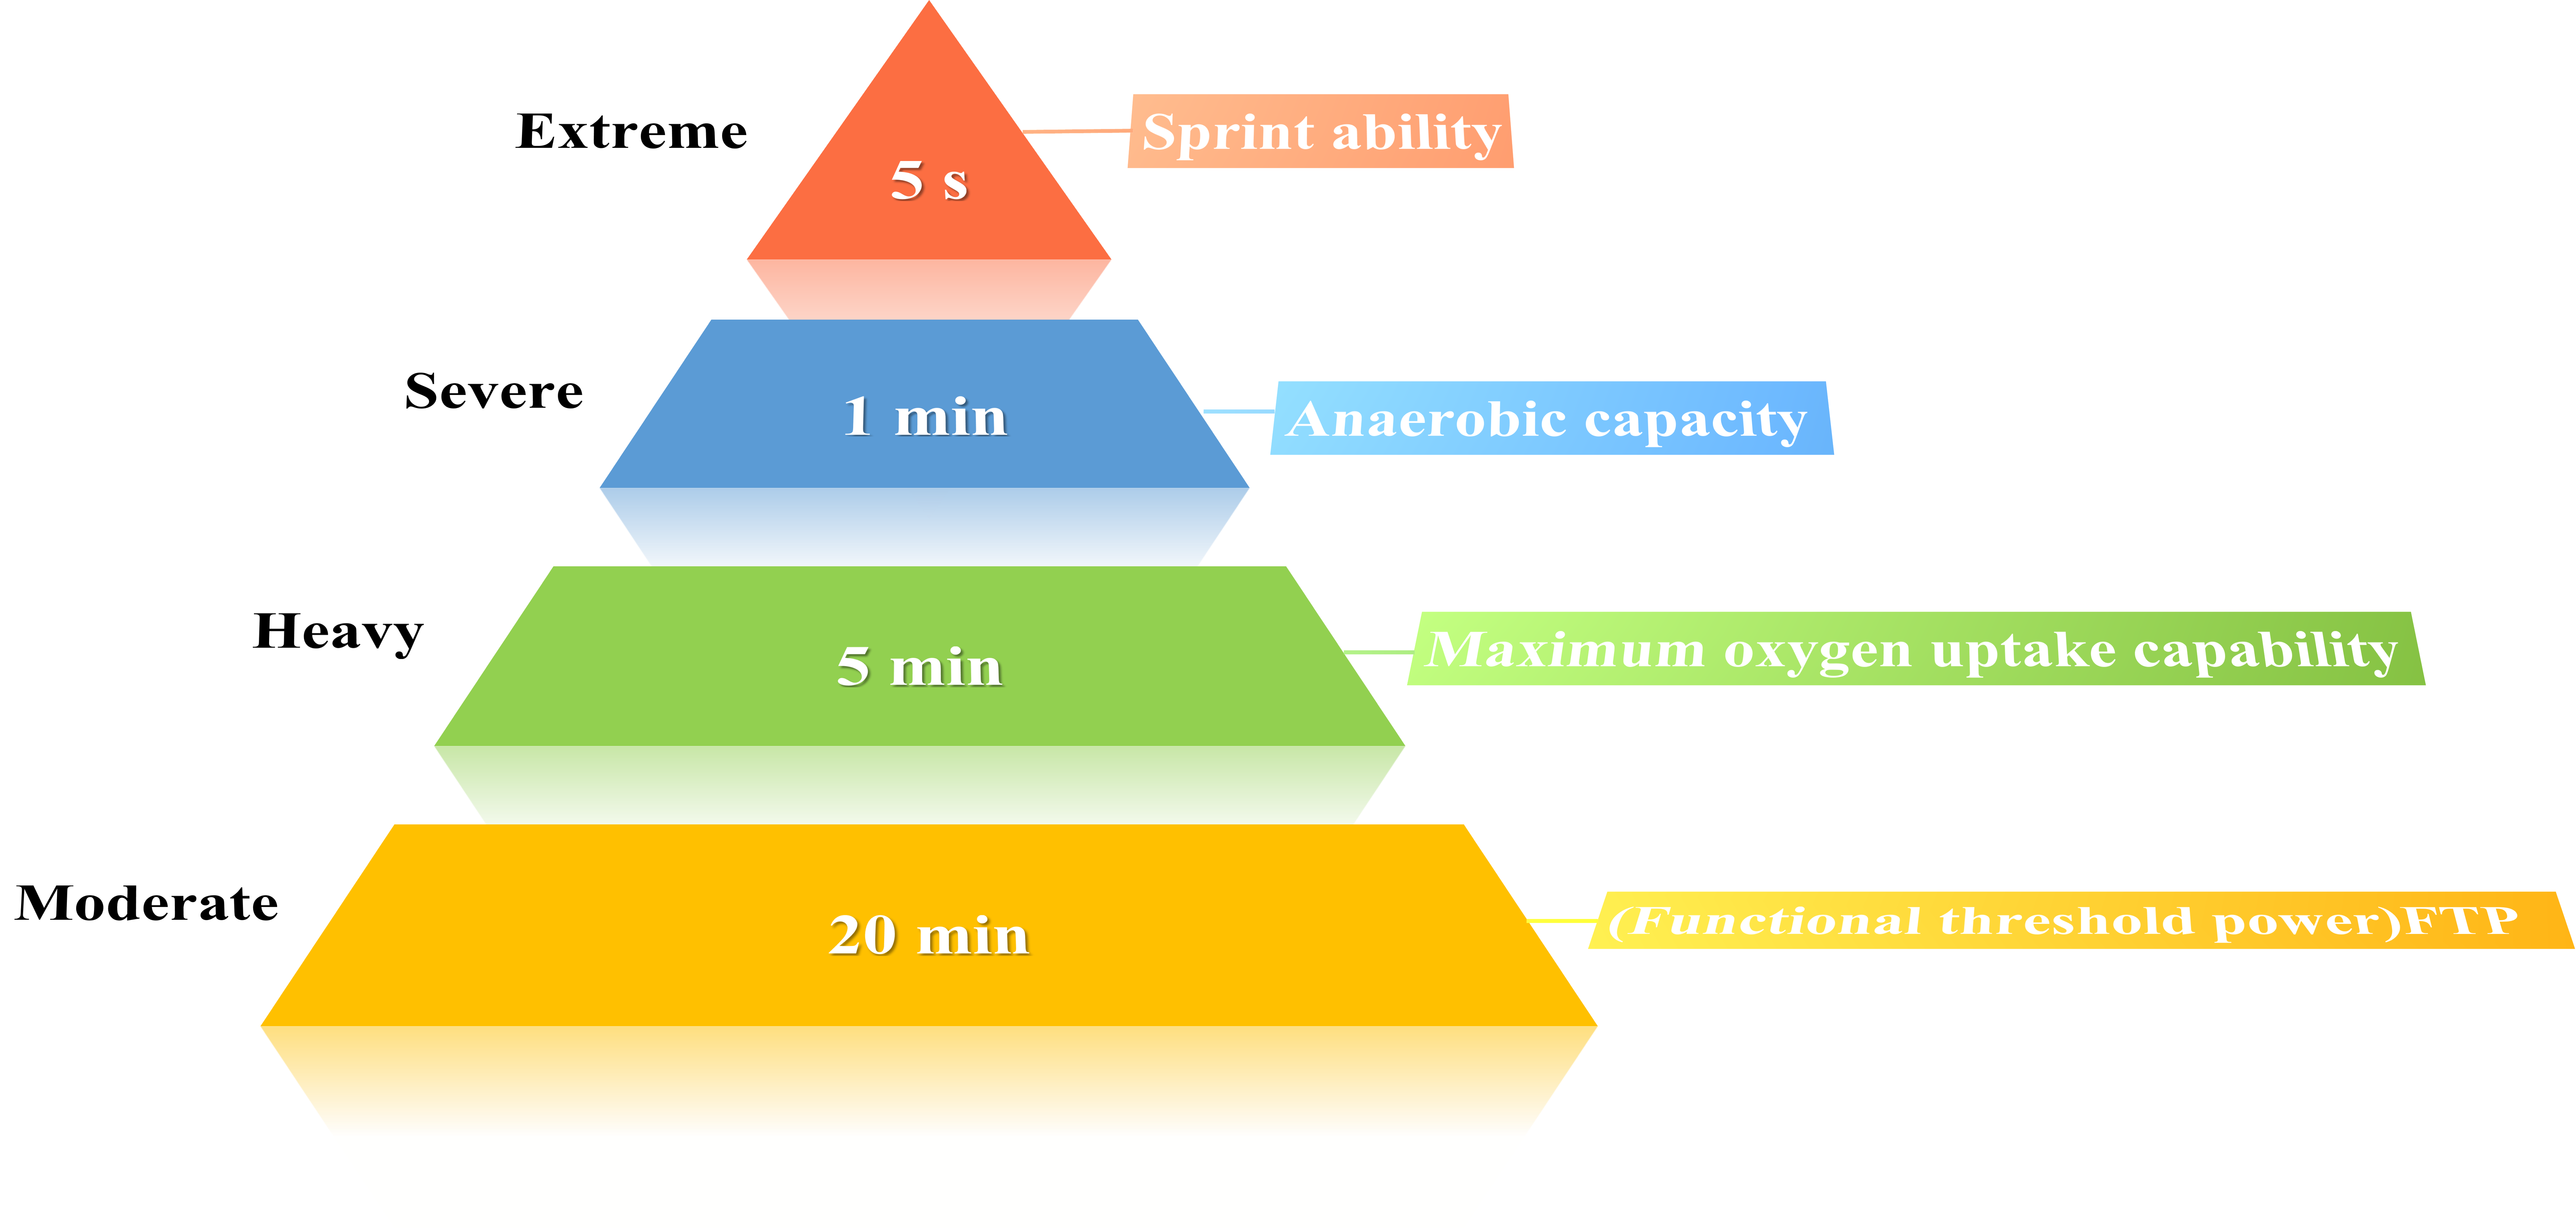
\includegraphics[width=0.9\linewidth]{image/pyramid}
\label{pyramid}
\end{wrapfigure}
	\par In this section, we establish the model of power curve, and consider people of different genders and types. 
	\par We first use the power profile chart to assess the ability of two types of rider briefly, which contains ability assessment in {\bf four domains}: {\bf extreme} intensity, {\bf severe} intensity, {\bf heavy} and {\bf moderate}, represented by {\bf 5s, 1 minute, 5 minutes and 20 minutes maximum power output} separately, as is shown on the left. Also, we plot the power curve of different athletes, showing the functional relationship  between maximal time and power output per weight. 